%
%   Prof. Dr. Julian Reichwald
%   auf Basis einer Vorlage von Prof. Dr. Jörg Baumgart
%   DHBW Mannheim
%
%
%	ACHTUNG: Für das Erstellen des Literaturverzeichnisses wird das modernere Paket biblatex
%			 in Kombination mit biber verwendet -- nicht mehr das ältere BibTex!
% 			 Bitte stellen Sie ggf. Ihre TeX-Umgebung
% 			 entsprechend ein (z.B. TeXStudio: Einstellungen --> Erzeugen --> Standard Bibliographieprogramm: biber)
%

\documentclass[
	12pt,
	BCOR=5mm,
	DIV=12,
	headinclude=on,
	footinclude=off,
	parskip=half,
	bibliography=totoc,
	listof=entryprefix,
	toc=listof,
	pointlessnumbers,
	plainfootsepline]{scrreprt}

%	Konfigurationsdatei einziehen
% !TEX root =  master.tex
% 		HYPERREF
%
\usepackage[
	hidelinks=true % keine roten Markierungen bei Links
]{hyperref}

% Zwei eigene Befehle zum Setzen von Autor und Titel. Ausserdem werden die PDF-Informationen richtig gesetzt.
\newcommand{\TitelDerArbeit}[1]{\def\DerTitelDerArbeit{#1}\hypersetup{pdftitle={#1}}}
\newcommand{\AutorDerArbeit}[1]{\def\DerAutorDerArbeit{#1}\hypersetup{pdfauthor={#1}}}

%		FONT AND INPUT ENCODING
%
\usepackage[T1]{fontenc}
\usepackage[utf8]{inputenc}

%		CALCULATIONS
%
\usepackage{calc} % Used for extra space below footsepline

%		LANGUAGE SETTINGS
%
\usepackage[ngerman]{babel} 	% German language
\usepackage[german=quotes]{csquotes} 	% correct quotes using \enquote{}

%\usepackage[english]{babel}   % For english language
%\usepackage{csquotes} 	% Richtiges Setzen der Anführungszeichen mit \enquote{}


%		BIBLIOGRAPHY SETTINGS
%
 \usepackage[backend=biber, autocite=footnote, style=authoryear, dashed=false]{biblatex} 	%Use Author-Year-Cites with footnotes
% \usepackage[backend=biber, autocite=inline, style=ieee]{biblatex} 	% Use IEEE-Style (e.g. [1])
% \usepackage[backend=biber, autocite=inline, style=alphabetic]{biblatex} 	% Use alphabetic style (e.g. [TGK12])

%%%% APA/Harvard-Style (bitte die nächten zwei Zeilen auskommentieren)
%\usepackage[backend=biber, style=apa]{biblatex} 	
%\DeclareLanguageMapping{german}{german-apa}

\DefineBibliographyStrings{ngerman}{  %Change u.a. to et al. (german only!)
	andothers = {{et\,al\adddot}},
}

%%% Uncomment the following lines to support hard URL breaks in bibliography 
%\apptocmd{\UrlBreaks}{\do\f\do\m}{}{}
%\setcounter{biburllcpenalty}{9000}% Kleinbuchstaben
%\setcounter{biburlucpenalty}{9000}% Großbuchstaben


\setlength{\bibparsep}{\parskip}		%add some space between biblatex entries in the bibliography
\addbibresource{bibliography.bib}	%Add file bibliography.bib as biblatex resource


%		FOOTNOTES 
%
% Count footnotes over chapters
\usepackage{chngcntr}
\counterwithout{footnote}{chapter}

%	ACRONYMS
%%%
%%% WICHTIG: Installieren Sie das neueste Acronyms-Paket!!!
%%%
\makeatletter
\usepackage[printonlyused]{acronym}
\@ifpackagelater{acronym}{2015/03/20}
  {%
    \renewcommand*{\aclabelfont}[1]{\textbf{\textsf{\acsfont{#1}}}}
  }%
  {%
  }%
\makeatother

%		LISTINGS
\usepackage{listings}	%Format Listings properly
\renewcommand{\lstlistlistingname}{Quelltextverzeichnis}
\lstset{numbers=left,
	numberstyle=\tiny,
	captionpos=b,
	basicstyle=\ttfamily\small}


%		EXTRA PACKAGES
\usepackage{lipsum}    %Blindtext
\usepackage{graphicx} % use various graphics formats
\usepackage[german]{varioref} 	% nicer references \vref
\usepackage{caption}	%better Captions
\usepackage{booktabs} %nicer Tabs
\usepackage{array}
%\newcolumntype{P}[1]{>{\raggedright\arraybackslash}p{#1}}
\usepackage{pdfpages}
\usepackage[figure]{hypcap}

%		ALGORITHMS
\usepackage{algorithm}
\usepackage{algpseudocode}
\renewcommand{\listalgorithmname}{Listingsverzeichnis }
\floatname{algorithm}{Algorithmus}
\usepackage{pdfpages}


%		FONT SELECTION: Entweder Latin Modern oder Times / Helvetica
\usepackage{lmodern} %Latin modern font
%\usepackage{mathptmx}  %Helvetica / Times New Roman fonts (2 lines)
%\usepackage[scaled=.92]{helvet} %Helvetica / Times New Roman fonts (2 lines)

%		PAGE HEADER / FOOTER
%	    Warning: There are some redefinitions throughout the master.tex-file!  DON'T CHANGE THESE REDEFINITIONS!
\RequirePackage[automark,headsepline,footsepline]{scrpage2}
\pagestyle{scrheadings}
\renewcommand*{\pnumfont}{\upshape\sffamily}
\renewcommand*{\headfont}{\upshape\sffamily}
\renewcommand*{\footfont}{\upshape\sffamily}
\renewcommand{\chaptermarkformat}{}

\clearscrheadfoot

\ifoot[\rule{0pt}{\ht\strutbox+\dp\strutbox}Watch Tycoon 2017]{\rule{0pt}{\ht\strutbox+\dp\strutbox}Watch Tycoon 2017}
\ofoot[\rule{0pt}{\ht\strutbox+\dp\strutbox}\pagemark]{\rule{0pt}{\ht\strutbox+\dp\strutbox}\pagemark}

\ohead{\headmark}


\begin{document}

%% BITTE GEBEN SIE HIER DEN TITEL UND DIE AUTORIN / DEN AUTOR DER ARBEIT AN!
\TitelDerArbeit{Watch Tycoon 2017}
%\AutorDerArbeit{Erika Musterfrau}

\begin{titlepage}
\begin{minipage}{\textwidth}
		\vspace{-2cm}
		\noindent  
		\centering 
\includegraphics{img/logo.jpg}
\end{minipage}
\vspace{1em}
\sffamily
\begin{center}
	\textsf{\large{}Duale Hochschule Baden-W\"urttemberg\\[1.5mm] Mannheim}\\[2em]
	\textsf{\textbf{\Large{}Systemanalyse - Fallstudie}}\\[3mm]
	\textsf{\textbf{\DerTitelDerArbeit}} \\[1.5cm]
	\textsf{\textbf{\Large{}Studiengang Wirtschaftsinformatik}\\[3mm] \textsf{Studienrichtung Software Engineering}}
	
	\vspace{5em}

\begin{minipage}{\textwidth}

\begin{tabbing}
	WIssenschaftlicher Betreuer:
	\hspace{0.5cm}\=\kill
	Kurs: \> WWI 16 SEA \\[1.5mm]
	Studiengangsleiter: \> Prof. Dr. Julian Reichwald  \\[1.5mm]
	Dozent: \> Hr. Gregor Tielsch  \\[1.5mm]
	Teammitglieder: \> Luisa Karl, \\ \> Rebekka Henn, \\ \> Miriam Wolf, \\ \> Ewald Anselm, \\ \> Tillmann Heß, \\ \> Erik Schmitt, \\ \> Nico Feil \\[1.5mm]
	Bearbeitungszeitraum: \> 28.08.2017 -- 17.11.2017
\end{tabbing}
\end{minipage}

\end{center}

\end{titlepage}

\pagenumbering{roman} % Römische Seitennummerierung
\normalfont

%--------------------------------
% Verzeichnisse - nicht benötige Verzeichnisse bitte auskommentieren / löschen.
%--------------------------------

%   Sperrvermerk
%\chapter*{Sperrvermerk}
Der Inhalt dieser Arbeit darf weder als Ganzes noch in Auszügen Personen außerhalb des Prüfungsprozesses und des Evaluationsverfahrens zugänglich gemacht werden, sofern keine anders lautende Genehmigung der Ausbildungsstätte vorliegt. 
\cleardoublepage


%	Kurzfassung
%\chapter*{Kurzfassung}
\begingroup
\begin{table}[h!]
\setlength\tabcolsep{0pt}
\begin{tabular}{p{3.5cm}p{11.9cm}}
Titel & \DerTitelDerArbeit \\
Verfasser/in: & \DerAutorDerArbeit \\
\end{tabular}
\end{table}
\endgroup

Hier können Sie die Kurzfassung der Arbeit schreiben.




%	Inhaltsverzeichnis
\tableofcontents

%	Abbildungsverzeichnis
%\listoffigures

%	Tabellenverzeichnis
%\listoftables

%	Listingsverzeichnis
%\lstlistoflistings

% 	Algorithmenverzeichnis
% \listofalgorithms

% 	Abkürzungsverzeichnis (siehe Datei acronyms.tex!)
%\clearpage
\chapter*{Abkürzungsverzeichnis}	
\addcontentsline{toc}{chapter}{Abkürzungsverzeichnis}


\begin{acronym}[RDBMS]
	\acro{DHBW}{Duale Hochschule Baden-Württemberg}
	\acro{RDBMS}{Relational Database Management System}
	\acro{BMBF}{Bundesministerium für Bildung und Forschung}	
\end{acronym}


%--------------------------------
% Start des Textteils der Arbeit
%--------------------------------
\clearpage
\ihead{\chaptername~\thechapter} % Neue Header-Definition
\pagenumbering{arabic}  % Arabische Seitenzahlen

% 	Einleitung
\clearpage
\chapter{Einleitung}
\section{Aufbau der Arbeit}
%\begin{tabbing}
%Vorlesung
%\hspace{0.2cm}\=\kill
%Vorlesung: \> Systemanalyse - Fallstudie \\
%Titel: \> Watch Tycoon 2017 
%\end{tabbing}
In dieser Arbeit wird die Erarbeitung einer Konzeption und Umsetzung eines Unternehmensplanspiels im Rahmen der Fallstudie beschrieben. Das Ziel dieser Arbeit ist die Entwicklung eines computergestützten Planspiels, auf dem die Spieler in Konkurrenz zueinander stehen und ein fiktiver Markt gebildet wird. Der Entwurf und die Entwicklung des Spiels bilden die Hauptaspekte dieser Arbeit. \\
Die Entwicklung wird in der Programmiersprache Java realisiert. Funktionen wurden zusätzlich in JavaScript geschrieben. Mit einem Tomcat-Webserver wird dann das Spiel lauffähig gemacht. \\
Betriebswirtschaftliche Aspekte werden in dem Spiel ebenfalls berücksichtigt. Dazu zählen zum Beispiel: variable Nachfrage der einzelnen Produkte, Betriebskosten oder Verkaufspreise. Die Marktveränderungen werden mittels eigen entwickeltem Algorithmus berechnet. \\
Die Entwicklung des grafischen User Interfaces wurde mit Hilfe von Bootstrap und HTML realisiert. Das Mock-Up, was ebenfalls in HTML statisch erstellt wurde, war dabei die Vorlage. \\ 
Mittels JUnit-Test werden die Szenario-Test durchgeführt und die Code-Coverage überprüft. Ziel hierbei ist eine Coverage > 65\%. Zudem werden die Use-Cases definiert und erläutert. \\
Des Weiteren wird die Projektorganisation vorgestellt, welche während dem Projekt eine wichtig Rolle gespielt hat. Hierbei wurde zusätzlich ein Meilenstein-Diagramm in \ref{fig:abb} auf Seite \pageref{meilenstein} verwendet um die einzelnen Meilensteine optisch darzustellen.\\
Zuletzt werden theoretische Verbesserungsmöglichkeiten aufgezeigt und ein Fazit über das gesamte Projekt gezogen.

\clearpage
\section{Herangehensweise}
Das Team setzt sich aus sieben Mitgliedern zusammen. Zu Beginn wurde in einem Kick-Off Meeting das Team bzw. die Industrie ausgewählt, aus welcher das Planspiel bestehen soll. Nach kurzer Überlegung konnte schnell in der Uhrenindustrie ein Nenner gefunden werden. \\
Auch bei der recht großen Anzahl an Teammitglieder konnte die Aufgaben sinnvoll aufgeteilt werden. So herrschte eine recht ausgewogene Balance, was die verschiedenen Schwerpunkte und Erfahrungen der Mitglieder betraf. Im Laufe des Projekte zeigte sich auch hierbei der Vorteil eines breiten technischen Portfolios. Dennoch konnten einige Problemstellung nicht mit dem reinen Wissen aus dem Studium abgedeckt werden. Ebenso waren Kenntnisse in der Mathematik und Wirtschaftswissenschaft gefragt um beispielsweise einen fiktiven Markt mit einem realistischen Algorithmus zu versehen.      

\section{Grundgedanke des Spiels}
Das Spiel \enquote{Watch Tycoon 2017} soll in einem rundenbasierten computergestützten Planspiel mit bis zu vier Spielern eine nahezu reale Unternehmenssimulation in einem Industriezweig darstellen. Der hierfür verwendet Industriezweig ist die Uhrenindustrie.\\
Der Spieler hat die Abteilungen Produktion, F\&E, Einkauf, Verkauf und Marketing zur Verfügung um eine bestmögliche Strategie auszuarbeiten und ein breites Spektrum an Varianz zu erhalten.\\
Der fiktive Markt soll mittels einem mathematischen Algorithmus so real wie möglich erstellt werden und den Mittelpunkt für Angebot und Nachfrage bilden.















% 	Grundgedanke des Spiels
\clearpage
\chapter{Grundgedanke des Spiels}
\section{Unternehmensbeschreibung}
\section{Fachkonzept}
\section{Mockup/UI}
\subsection{Mockup}
\subsection{Finales UI}

% 	Industriezweig Uhr
\clearpage
\chapter{Die Uhrenindustrie}
Die Schweiz ist derzeit das Land mit den meisten Uhrenexporten. Gemessen an den Exporten ist die Uhrenindustrie innerhalb der Schweiz jedoch nur die drittgrößte Industrie. Weltweit gefolgt wird die Schweiz Hongkong und China. 
In den 1970er und 1980er Jahren erhielt die klassische schweizer Uhrenindustrie Konkurrenz durch die Entstehung der elektrischen Uhren und den asiatischen Markt. Nachdem sie sich bis 2015 wieder etwas erholen konnte und die Exporte von 4,3 Milliarden Franken im Jahr 1986 auf 21,5 Milliarden im Jahr 2015. 
Mittlerweile schaffen es vor allem die Großmarken, sich gegen die neue Konkurrenz der Smart Watches durchzusetzen, indem sie entweder hochwertige Luxusuhren herstellen, die als Schmuckstück und Statussymbol dienen oder indem sie selbst Smart Watches entwickeln.


% 	Spielplan
\clearpage
\chapter{Spielplan}
(NF) Spielplan "Watch Tycoon" \\
Anzahl der Spieler: 2-4 \\
Spielverfahren: Rundenbasiertes Strategiespiel mit Hot-Seat Verfahren \\
Maximal Anzahl der Spielrunden (insgesamt): 10 Runden \\
\\
Jeder Spieler hat zu Beginn ein Grundkapital von 1.000.000 EURO. Zu Beginn des Spiels muss eine Uhr aus den Segmenten Masse, Öko oder Luxus ausgewählt werden. Je nach Auswahl stehen verschiedene Ausstattungsmerkmale zur Verfügung zudem wird bei der Auswahl des jeweiligen Segments ein unterschiedlicher Betrag zu Beginn abgezogen. Wenn alle Spieler an der Reihe waren, werden die gemachten Änderungen auf den fiktiven Markt übertragen. \\ 
\\
Einkauf:\\
Im Bereich Einkauf können Verbesserungen für die jeweiligen Merkmale gekauft werden. Dadurch werden Kosten gesparte und es entsteht eine Art Rabatt für das jeweilige Merkmal. \\
\\
Vertrieb: \\
Hier lassen sich der Verkaufspreis und die geplante Absatzmenge für die maximal drei Uhren eingeben.\\
\\
Marketing:\\
Im Marketing dreht sich alles um das Bekanntmachen einer neuen Uhr und des Unternehmens. Hierfür stehen jeweils drei Werbemöglichkeiten zur Verfügung. Aber Achtung: Eine Werbekampagne muss sich nicht immer gut auswirken!\\ 
\\
Produktion: \\
In der Produktion können durch Zukäufe von Produktionsstraßen (maximal zwei weitere Produktionsstraßen möglich) entweder weitere Segmente eröffnet werden oder eine Kostensenkung durch ein bereits vorhandenes Segment erzielt werden. Des Weiteren können für die vorhandenen Produktionsstraßen Erweiterungen gekauft werden (maximal drei weitere möglich) um ebenfalls die Kosten zu senken. \\ 
\\
\\
Forschung\&Entwicklung:\\
Die F\&E (Forschung\&Entwicklung) ist für die Erforschung von besseren Ausstattungsmerkmalen der jeweiligen Segmente zuständig. Durch das Erforschen der zusätzlichen Merkmale wird die Uhr hochwertiger und kann für mehr Geld verkauft werden.\\
\\
Die Unternehmensabteilungen Marketing, Verkauf, Einkauf, Produktion und F\&E sind ab Runde 1 verfügbar.\\
\\
Der Markt dient als Informationsinstrument für jeden Spieler. Dabei kann der Spieler die Nachfrage und das Marktvolumen einsehen und gegen Geld einmalig den Markt analysieren lassen. Sofern sich ein Spieler für die Produktion der Öko-Uhr entscheidet, erhält dieser zusätzlich einen Bonus, der später in der Endwertung mit einfließt.\\ 
\\
Ziel des Spiels/Gewinnbedingung:\\
Ziel des Spiels ist es nach Ablauf der 10 Spielrunden den größten Gewinn erzielt zu haben.




% 	Abteilungen
\clearpage
\chapter{Abteilungen}

\section{Produktion}
Die Abteilung Produktion stellt für den Spieler die wichtigsten Funktionen zur Herstellung seiner Uhr zu Verfügung dar.\\ 
Der Spieler hat in dieser Abteilung zwei Möglichkeiten seine Produktionsstraßen auszubauen und seine Produktion um die zwei weiteren Segmente zu erweitern:
\begin{enumerate}
	\item Erweiterung der bestehenden Produktionsstraße
\begin{itemize}
	\item  
\end{itemize}
	\item Erweiterung um neues Marktsegment
\begin{itemize}
	\item  
\end{itemize}
	\item Ausbau bestehender Produktionsstraße(n)
\begin{itemize}
	\item  
\end{itemize}
\end{enumerate}
    
\section{Forschung\&Entwicklung}

\section{Marketing}

\section{Verkauf}

\section{Einkauf}\label{sec:einkauf}
Der Einkauf sollte dem Spieler zunächst drei Optionen bieten:
\begin{enumerate}
\item Der Einkauf von Rohstoffen \par
Da Uhren oft aus sehr individuellen Materialien bestehen, sollte es hier eine Liste möglicher Rohstoffe geben, die je nach Marktsegment ausgewählt werden können.
\begin{itemize}
\item	Holz	\\
\item	Textilien	\\
\item	Kunststoffe	\\
\item	Edelstahl \\
\item	Reintitan \\
\item	Aluminium \\
\item	High-Tech-Keramik \\
\item	Gold, Silber, Platin
\item Edelsteine und Perlen \\
\item Leder, Wildleder, Krokodilsleder \\
\item	Fischhaut
\item	Glas \\
\end{itemize}
\item Der Einkauf von halbfertigen und fertigen Erzeugnissen \par
Da die Hauptbestandteile einer Uhr aus vielen kleinen Einzelteilen bestehen, werden diese meist durch Fremdbezug erworben. Bei dieser Option sollen also die bereits hergestellten Hauptbestandteile eingekauft werden.
\item Die Eigenproduktion durch beispielsweise einen eigenen Holzanbau
\end{enumerate}

Da die zweite Option auch in der Realität weit verbreitet ist, wurde beschlossen, dass sich auf die Auswahl eines Armbands, eines Gehäuses und eines Uhrwerks beschränkt wird.

Des Weiteren sollte es die Möglichkeit geben, Lieferanten gezielt auswählen zu können und dabei auf Faktoren wie Kosten, Regionalität und Transportmittel zu achten.
Diese Option wurde aufgrund des hohen Aufwands jedoch nicht in das Spiel übernommen.

Auch Skonti und Rabatte sollen im Einkauf möglich sein. Sie sind vor allem mengenabhängig und richten sich nicht nach einzelnen Lieferanten.

Für die Produkte, die im Ökosegment angeboten werden können, sollte es beim Einkauf zusätzliche Informationen zu Siegeln wie beispielsweise dem Blauer Engel für Leder und Fairtrade für Gold und Edelsteine geben.
Diese Möglichkeit kommt als Erweiterung des Spiels in Frage, da sie zunächst nicht spielentscheidend oder notwendig für die Funktionalität ist.



% 	Architektur/tech. Grundlagen
\clearpage
\chapter{Architektur}
In diesem Kapitel wird der technische Aufbau des Spiels beschrieben. Hierbei wird auf die verwendete Architektur sowie die zugrunde liegenden Designentscheidungen eingegangen.

\section{Einflussfaktoren für Architektur}
Die Maßgebenden Einflussfaktoren für die Entscheidung der verwendeten Softwarearchitektur, sind neben dem im Team vorhanden Know-How bezüglich Programmiersprachen und Unit-Tests, die eigenen Anforderungen an die optische Repräsentation des Spiels. Nach einer Aufnahme der Kenntnisse der Teammitglieder war schnell ersichtlich, dass die Programmiersprache Java am verbreitetsten ist und sich in Bezug auf Unit-Tests auch hier die größte Übereinstimmung findet.

Der in der Vorlesung zur Fallstudie vorgestellte Tomcat-Server bietet die Möglichkeit, für ein in Java geschriebenes Fachkonzept ein Userinterface auf HTML-Basis bereitzustellen. Da die in Java zur Verfügung stehende SWING-Bibliothek nicht die gewünschten optischen Resultate erzielt, wurde diese schnell ausgeschlossen.

\section{Übersicht über technischen Aufbau}
Aus den zuvor genannten Beweggründen ergab sich schnell der in \ref{fig:abb} 
\begin{figure}[!h]
	\centering
	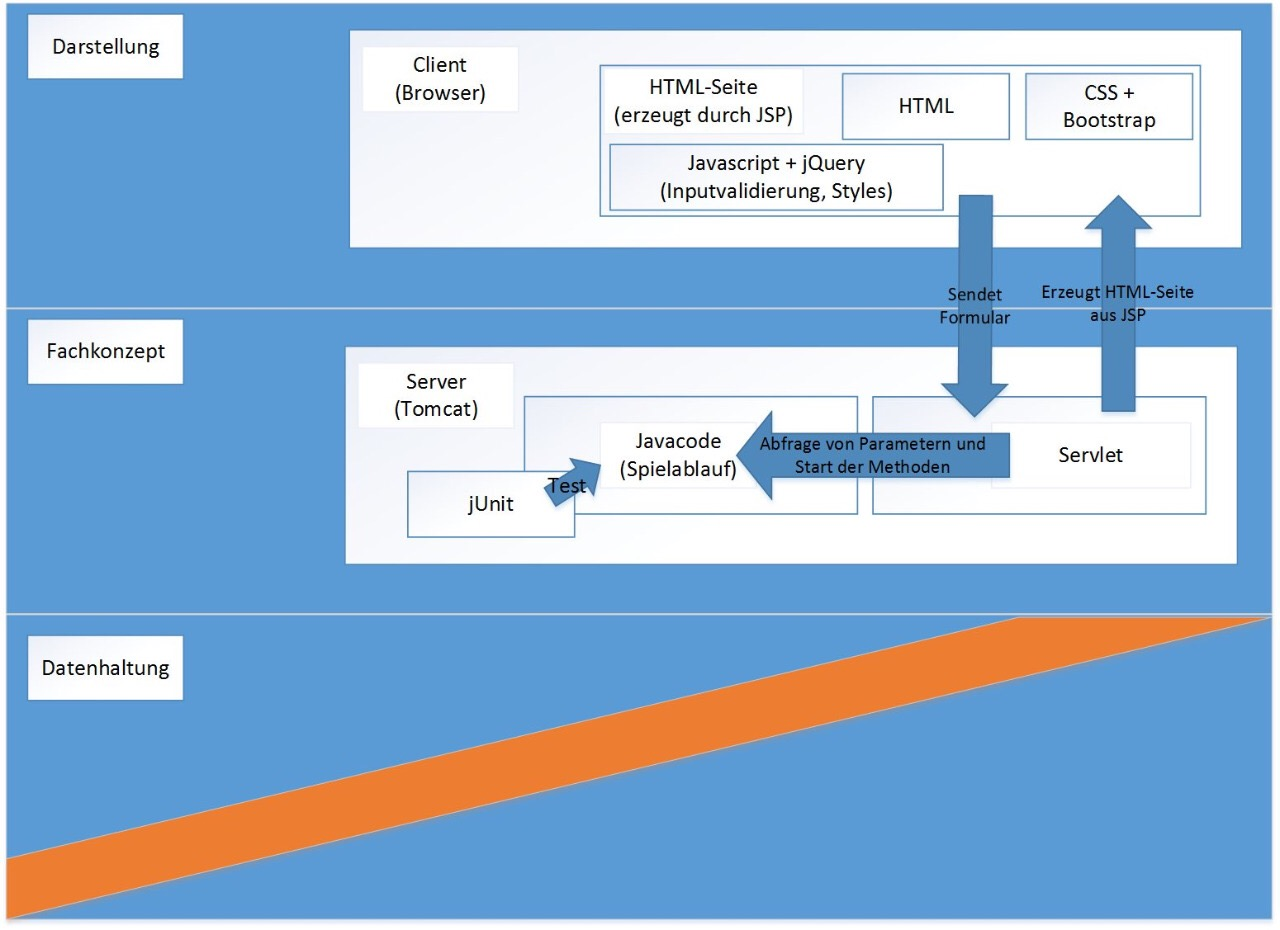
\includegraphics[scale=0.2]{img/3-schichten-modell.jpeg}
	\label{fig:abb} 
	\caption{3-Schichten-Modell} 
\end{figure}
dargestellte Aufbau der Software. Im ersten Schritt zur Gliederung der Architektur wurde die aus dem Studium bekannte 3-Schichten-Architektur zugrunde gelegt. Die Software wird hierbei in die ebenen Datenhaltung, Fachkonzept sowie Darstellung untergliedert. Bei den vorgegebenen Anforderungen an die Fallstudie, ist eine Datenhaltung als optional angegeben. Zur Reduzierung des Programmieraufwandes wurde auf eine Datenbankanbindung oder sonstige Datenhaltung verzichtet.

Zur Umsetzung des Fachkonzeptes wird auf die Programmiersprache Java gesetzt. Wobei die gesamte Spiellogik so umgesetzt ist, dass hierauf ein beliebiges Userinterface aufgesetzt werden kann. Zum Testen des Fachkonzepts kommt JUnit zum Einsatz. Da als Userinterface eine Webseite dienen soll, wird das Fachkonzept nicht in einer lokalen JVM sondern auf einem Webserver ausgeführt. Der zum Einsatz kommende Tomcat-Server kann sowohl den Java-Code des Fachkonzepts ausführen, als auch über die gewünschte Webseite Eingaben des Anwenders entgegen nehmen, bzw. entsprechende Ausgaben zurückgeben. Die dabei zum Einsatz kommenden Techniken werden in den folgenden Kapiteln näher erläutert.

Bei der Darstellungsebene des Spiels werden die gestalterischen Möglichkeiten von HTML, CSS sowie JavaScript genutzt, indem der Tomcat-Server für den Anwender eine entsprechende Webseite als Userinterface zur Verfügung stellt. Die Bedienung des Spiels erfolgt somit für den Anwender in einem Webbrowser.

Folglich ergibt sich, neben einer logischen Trennung von Fachkonzept und Darstellung, eine technische Trennung, in Form einer Client-Server-Architektur. Auf dem Server wird die Spiellogik ausgeführt, eine dynamische Webseite generiert und auf Eingaben des Anwenders gewartet. Im Browser des Clients wird hingegen die dynamisch generierte Webseite mit den aktuellen Werten des Spielstandes angezeigt, als auch eine Eingabemöglichkeit zur Ausführung von gewünschten Spielaktionen geboten.

\section{Laufzeitumgebung}
Da die Spiellogik in Java programmiert ist, wird zur Ausführung des Programms eine Java-Laufzeitumgebung benötigt. Während der Entwicklung wird hier im speziellen die Java Runtime Environment in Version 8 verwendet. Eine weitere wichtige Komponente ist der Servlet-Container. Die an den Server übermittelten Eingaben, in Form von Http-Requests, werden vom Webserver entgegen genommen und an den Servlet-Container weitergeleitet. Dieser verarbeitet die Requests und leitet diese an das Servlet, welches im folgenen Kapitel näher beschrieben wird, weiter. Zur Bereitstellung einer serverseitigen Java-Laufzeitumgebung, als auch einem Servlet-Container, dient der bereits angesprochene Tomcat-Server von Apache.

\section{Java Servlets}\label{sec:Servlets}
Auf dem bereits erwähnten Tomcat-Server wird eine Instanz der Klasse Servlet ausgeführt. Hierüber wird es ermöglicht, auf Eingaben des Anwenders zu reagieren und entsprechende Rückgaben auszuliefern. Die Kommunikation zwischen Server und Client erfolgt hierbei mittels Http-Requests. In diesem Fall wird die doPost()-Methode der Klasse HttpServlet überschrieben und mit den gewünschten Funktionalitäten versehen.

Der Aufruf der Methode erfolgt von Seiten des Clients durch absenden eines HTML-Formulars. Im Kapitel \ref{UI} auf Seite \pageref{UI} wird hier näher drauf eingegangen. Innerhalb der doPost()-Methode können über das request-Objekt auf die vom Anwender getätigten Eingabeparameter zugegriffen werden. Aufgrund der Eingaben des Anwenders werden die entsprechenden Methoden der Spiellogik mit den benötigten Übergabeparametern aufgerufen. Bei einem ggf. stattzufindenden Seitenwechsel im Browser werden weiterhin entsprechende Übergabeparameter dem request-Objekt hinzugefügt und die neue Seite unter Mitgabe des Objekts aufgerufen.

Zur weiteren Vereinfachung des Programmieraufwandes wird innerhalb der Servlet-Instanz nicht nur die Kommunikation mit dem Client koordiniert, sondern auch eine Instanz des Spiels erzeugt. Alle innerhalb der doPost()-Methode getätigten aufrufe bezüglich der Spiellogik werden somit an die Instanz des Spiels übergeben. Auch wenn auf abstrakter Ebene das Servlet und die Spiellogik als zwei getrennte Elemente betrachten werden, ist die Spielinstanz real gesehen eine Instanz innerhalb des Servlets.

\section{JavaServer Page}
Wie im Kapitel \ref{sec:Servlets} auf Seite \pageref{sec:Servlets} beschriebenen werden in der doPost()-Methode neue Webseiten unter Mitgabe des request-Objekts aufgerufen. Da eine nur mit HTML erstellte Seite mit dem request-Objekt nicht umgehen kann, kommt zur Erstellung der Webseite JavaServer Page bzw. Expression Language zum Einsatz. Der Einsatz beider beschränkt sich jedoch innerhalb dieses Projektes auf die Angabe des Ziels des HTML-Formulars sowie als Platzhalter für Variablen zur dynamischen Erstellung von Seiteninhalten.

Die Webseite wird wie gewohnt mit HTML erstellt, wobei die dynamisch zu erstellenden Inhalte im Quellcode durch Value Expressions ( \$\{ Value \} ) ersetzt werden. Beim Aufruf der Seite innerhalb der doPost()-Methode werden die Value Expressions mit den gleichnamigen Parametern aus dem request-Objekt ersetzt und der so entstehende HTML-Code an den Browser des Clients ausgeliefert. In diesem Projekt werden hierdurch vor allem Textinhalte innerhalb von HTML-Elementen generiert bzw. bestimmte Werte dem Class-Attribut der HTML-Elemente hinzugefügt.

\section{User Interface}\label{UI}
Zur Erstellung des Userinterface kommen überwiegend die für Webanwendungen üblichen Technologien in Form von HTML5, CSS3 und JavaScript sowie aktuell gängige Frameworks zum Einsatz. Die logische Strukturierung der Seiten erfolgt mittels der Auszeichnungsprache HTML. Die Gestaltung des Userinterface in Bezug auf Layout, \enquote{Look and Feel} erfolgt überwiegend mittels CSS3 sowie zur Reduzierung des Programmieraufwands mittels dem CSS-Framework Bootstrap. JavaScript sowie das JS-Framework jQuery werden zur logischen Validierung von Benutzereingaben siwue zur Umsetzung einiger kontextbezogener optischer Effekte bzw. Layoutumgestaltungen, welche sich mittels CSS schwierig oder nicht umsetzten lassen.

Die Aufteilung des Userinterface auf mehrere JSP-Dokumente ergibt sich in erster Linie aus an den Server zu schickenden Formularen und dem im Servlet definierten Requests. Für jedes zu versendende Formular wird ein eigenes JSP-Dokument verwendet. Die Formulare wiederum repräsentieren logische Spielabschnitte.

Die Startseite beinhaltet eine Auswahlmöglichkeit für die gewünschte Spieleranzahl sowie einen Button zum Start des Spiels. Mit Klick auf den Start-Button wird das Formular an das Servlet gesendet. Es wird das Spiel-Objekt mit der ausgewählten Anzahl an Spielern erzeugt und anschließend die erste Spielrunde mit dem ersten Spielzug des ersten Spielers begonnen.

In der ersten Spielrunde eines jeden Spielers wird dieser auf eine weitere Seite geführt. Hier hat der Spieler zu entscheiden auf welche Sparte bzw. welches Marktsegment sein Unternehmen zu Beginn ausgerichtet ist. Mit Versandt des Formulars an den Server erfogt in der doPost()-Methode eine Abfrage welcher Button dsa Formular versendet hat, genauer gesagt, welcher Button zum aktuellen Zeitpunkt einen Value dem Http-Request mitgegeben hat. Dementsprechend erfolgt die Ausführung der entsprechenden Methoden im Fachwerk zum Freischalten der ausgewählten Sparte beim jeweiligen Spieler und Erzeugung der ersten Uhr für das ausgewählte Marktsegment. Der letzte Schritt in diesem Abschnitt ist dann die Weiterleitung des Spielers an die für ihn benötigten Auswahl- wowie Anzeigeelemente für eine Spielrunde.

Aufgrund des Quellcodeumfangs zur Darstellung der Eingabemaske, für die vom Spieler während eines Spielzugs zu tätigenden Aktionen, bzw. zur Anzeige seiner aktuellen Spielinformationen, ist der entsprechende Quellcode auf mehrere Dateien aufgeteilt. Eine Datei beinhaltet die Navigationselemente sowie das \enquote{Grundgerüst} der Seite. Die durch die Navigationselemente umschaltbare Spielelemente sind zur besseren Übersicht über den Quellcode in weitere Dateien ausgelagert. JSP bietet hier die Möglichkeit die ausgelagerten Dateien mittels jsp:include einzubinden. Während der serverteitigen Kompilierung werden aus den einzelnen Dokumenten ein einzelnes Dokument für den Client bzw. dessen Browser erstellt. 

Mittels Buttons kann der Spieler wählen, welche Aktionen in der aktuellen Spielrunde durchgeführt werden sollen. Ein Script, mittels JavaScript umgesetzt, übergibt an das jeweilige versteckte Inputfeld einen entsprechenden Wert.
Nach Tätigung aller während der aktuellen Spielrunde gewünschten Spielaktionen, kann der Spieler den Button \enquote{Runde beenden} betätigen. Die in den versteckten Inputfeldern gesammelten Spielaktionen werdenüber das HTML-Formular in Form eines Http-Requests an die doPost()-Methode innerhalb des Servlet-Objekts weitergeleitet. Innerhalb der Methode wird geprüft welche Buttons angeklickt wurden und die äquivalenten Methoden im Fachkonzept ausgeführt sowie die Methode zum Wechsel des Spielers aufgerufen. Am Ende dieses Abschnittes wird eine neue Seite mit Anzeige der aktuellen Runde sowie des nächsten Spielers angezeigt. Dieser kann gemäß des Hot-Seat-Verfahrens den Platz am Bildschirm einnehmen und seine Runde beginnen. Zum Ende der letzen Spielrunde wird das letzte Dokument zur Darstellung des Gewinners, bzw. der Gewinnreihenfolge der Spieler angezeigt. Unterhalb der Gewinneranzeige gibt es die Möglichkeit ein neues Spiel zu starten.

Neben der Dokumentenstruktur ist die Verwendung von CSS-Regeln und CSS-Klassen ein weiteres wichtiges Element der Umsetzung des Userinterface. Die CSS-Regeln sind derart gestaltet, dass je nachdem was der Spieler freigeschalten bzw. nicht freigeschaltenen hat, eine entsprechende optische Darstellung erfolgt. Als Selektoren kommen hierbei überwiegend CSS-Klassen zum Einsatz. In den entsprechenden HTML-Elementen sind im Value-Bereich des class-Attributs Value Expressions eingebettet. Je nach freigeschaltenen Spielelementen werden im request-Objekt entsprechende Werte hinterlegt. Beim Kompilieren der Webseite werden die Value Expressions ggf. durch die entsprechenden Werte im request-Objekt ersetzt und somit die definierte CSS-Klasse beim HTML-Element definiert. Im Spielerobjekt hinterlegte Werte wie zum Beispiel das aktuelle Kapital oder der Warenbestand der Uhren werden auf die gleiche Art und Weise der Webseite übergeben. Die Value Expressions sind dann jedoch so im Quellcode plaziert, dass diese als Text ausgegeben werden und nicht dem jeweiligen Element als class-Atribute mitgegeben werden.

\clearpage
\chapter{Entwickungsumgebung}
\section{Eclipse JAVA EE IDE}
Eclipse ist eine Programmierumgebung als Entwicklungswerkzeug von Software und Programmen aller Art. Es gibt eine Vielzahl von kommerziellen und kostenlosen Erweiterungen. Unter Eclipse ist es möglich nahezu jede Programmiersprache zu entwickeln. Für das Projekt wurde lediglich die Programmiersprache Java für die Logik der Simulation verwendet. Als integrierte Entwicklungsumgebung umfasst Eclipse nicht nur einen Texteditor zum erstellen des Quellcodes, sondern viele weiterere für die Softwareentwicklung benötigten oder hilfreichen Programme bzw. Funktionen. Diese lassen sich dank des modularen Aufbaus von Eclipse in beliebiger Kombination hinzufügen, oder man verwendet eine der für bestimmte Anwendungsfälle bereits vorkonfigurierten Versionen. Aufgrund der Verwendung einer Server-Client-Architektur unter Verwendung von Java Servlets, bietet es sich an, die entsprechende Version Eclipse JAVA EE IDE zu verwenden. Diese Version beinhaltet gleich die benötigten Komponenten, um den Tomcat-Server in die IDE einbinden zu können. Das Testen einzelner Funktionen kann somit innerhalb der Entwicklungsumgebung erfolgen und eine separate Verwaltung eines Webservers zu Testzwecken ist somit nicht erforderlich.
\section{Git}
Bei Git handelt es sich um eine freie Software zur Versionsverwaltung. Git ist Open Source und lediglich per Kommandozeile verfügbar. Dennoch gibt es bereits unzählige grafische UIs, die Git vereinfachen und seine Befehle grafisch darstellen (beispielhaft dafür: Sourcetree, GitHub Desktop oder TortoiseGit) . Git wird auch von zahlreichen Großprojekten verwendet, darunter Android, LibreOffice oder jQuery. 
\section{GitHub}
GitHub ist der webbasierte Online-Dienst, welcher Entwicklungsprojekte auf einem Server bereitstellt und somit Filehosting betreibt. Grundsätzlich ist es nicht anderes als Git, eben nur nicht lokal, zudem bringt GitHub seinen eigenen grafischen UI Client namens GitHub Desktop mit. Ein grafischer Client wurde in diesem Projekt nicht mitgliederübergreifend eingesetzt. Weiterhin bieten viele Entwicklungsumgebungen wie auch Eclipse eine integrierte Möglichkeit auf die gehosteten Softwarerepositories zuzugreifen. Auch diese Lösung kam im Team zum Teil in Einsatz.
\section{LaTeX}
Für die Erstellung der Dokumentation wurde das Softwarepaket LaTeX genutzt. Als Editor wurden überwiegend TeXstudio oder der zur Softwareentwicklung gedachte Texteditor Atom eingesetzt.\\
LaTeX ist ein Softwarepaket, welches die Benutzung des Textsatzsystems TeX mit Hilfe von Makros vereinfacht.
LaTeX ist die populärste Methode TeX zu verwenden.
TeXstudio ist ein plattformunabhängiger Editor zur Erstellung von genannten LaTeX Dokumenten.\\
Beide sind Open-Source und kostenlos. Neben TeXstudio gibt es noch eine Vielzahl an weiteren Editoren, speziell für LaTeX Dokumente.



% 	Test
\clearpage
\chapter{Qualitätssicherung mittels JUnit-Tests}
\section{Vorgehensweise}
Zunächst wurde die Funktionalität der Methoden der Unternehmenssimulation anhand einfacher Konsolenausgaben durch die Entwickler unseres Teams getestet. Diese Art der Tests kann als Entwicklertest eingestuft werden. Die Entwicklertests werden in der Regel vom Entwickler selbst durchgeführt und dienen zur Überprüfung von Zwischenergebnissen und einzelnen Codezeilen. \par
Nachdem die Funktionalität der Methoden überprüft und gegebenenfalls angepasst wurde, konnte mit dem Schreiben von JUnit-Tests begonnen werden. Unit-Tests, auch Modultests genannt, überprüfen einzelne isolierte Komponenten wie beispielsweise Methoden. Dadurch ist es möglich, Fehler schnell und einfach zu erkennen. Eine Änderung muss oft nur an einer Stelle vorgenommen werden, da die Methoden unabhängig voneinander sein sollen. Da sich in umserem Projekt viele Methoden aufeinander aufbauen, war es nicht möglich, alle Methoden isoliert zu testen. Es existiert jedoch immer ein Test, der zunächst die Grundlage testet, zum Beispiel einen Spieler zu erstellen. Diese Methode wird dann in nachfolgenden Tests erneut aufgerufen, um eine logische Einheit abbilden zu können. Das Testen einer sinnvollen Einheit ist uns wichtiger, als ein isoliertes Detail zu testen, das aber in dieser Form kein Mehrwert bringt.

%% Codebeispiel (erforsche Uhr)? zum verdeutlichen vom aufeinander aufbauen

\section{Testergebnisse}

%	Use Cases
\clearpage
\chapter{Use-Cases}
\section{1. Case}
\section{2. Case}
\section{3. Case}

% 	Projektorganisation
\clearpage
\chapter{Projektorganisation}
\section{Aufgabenverteilung}
Wie bereits in \ref{sec:herangehensweise} erläutert wurde, war das Projektteam sehr gut ausbalanciert und brachte ein breites Spektrum an technischen und wirtschaftlichen Verständnis mit. Um die konkrete Aufgabenteilung darzustellen, sind nachfolgende alle Aufgaben und deren Bearbeiter beschrieben. 
\begin{enumerate}
	\item Coding
	\begin{itemize}
		\item Miriam Wolf, Erik Schmidt, Ewald Anselm
	\end{itemize} 
	\item JUnit-Tests: Erstellung, Realisierung und Implementierung
	\begin{itemize}
		\item Rebekka Henn, Luisa Karl
	\end{itemize} 
	\item Coding Layout: Erstellung, Realisierung und Implementierung
	\begin{itemize}
		\item Ewald Anselm, Erik Schmidt
	\end{itemize} 
	\item Markt Algorithmen: Erstellung, Realisierung und Implementierung
	\begin{itemize}
		\item Tilman Heß
	\end{itemize} 	
	\item Dokumentation und Präsentation
	\begin{itemize}
	\item Nico Feil
	\end{itemize}
\end{enumerate}
\clearpage
\section{Meilensteine}\label{sec:meilenstein}
\begin{figure}[!h]
	\centering
	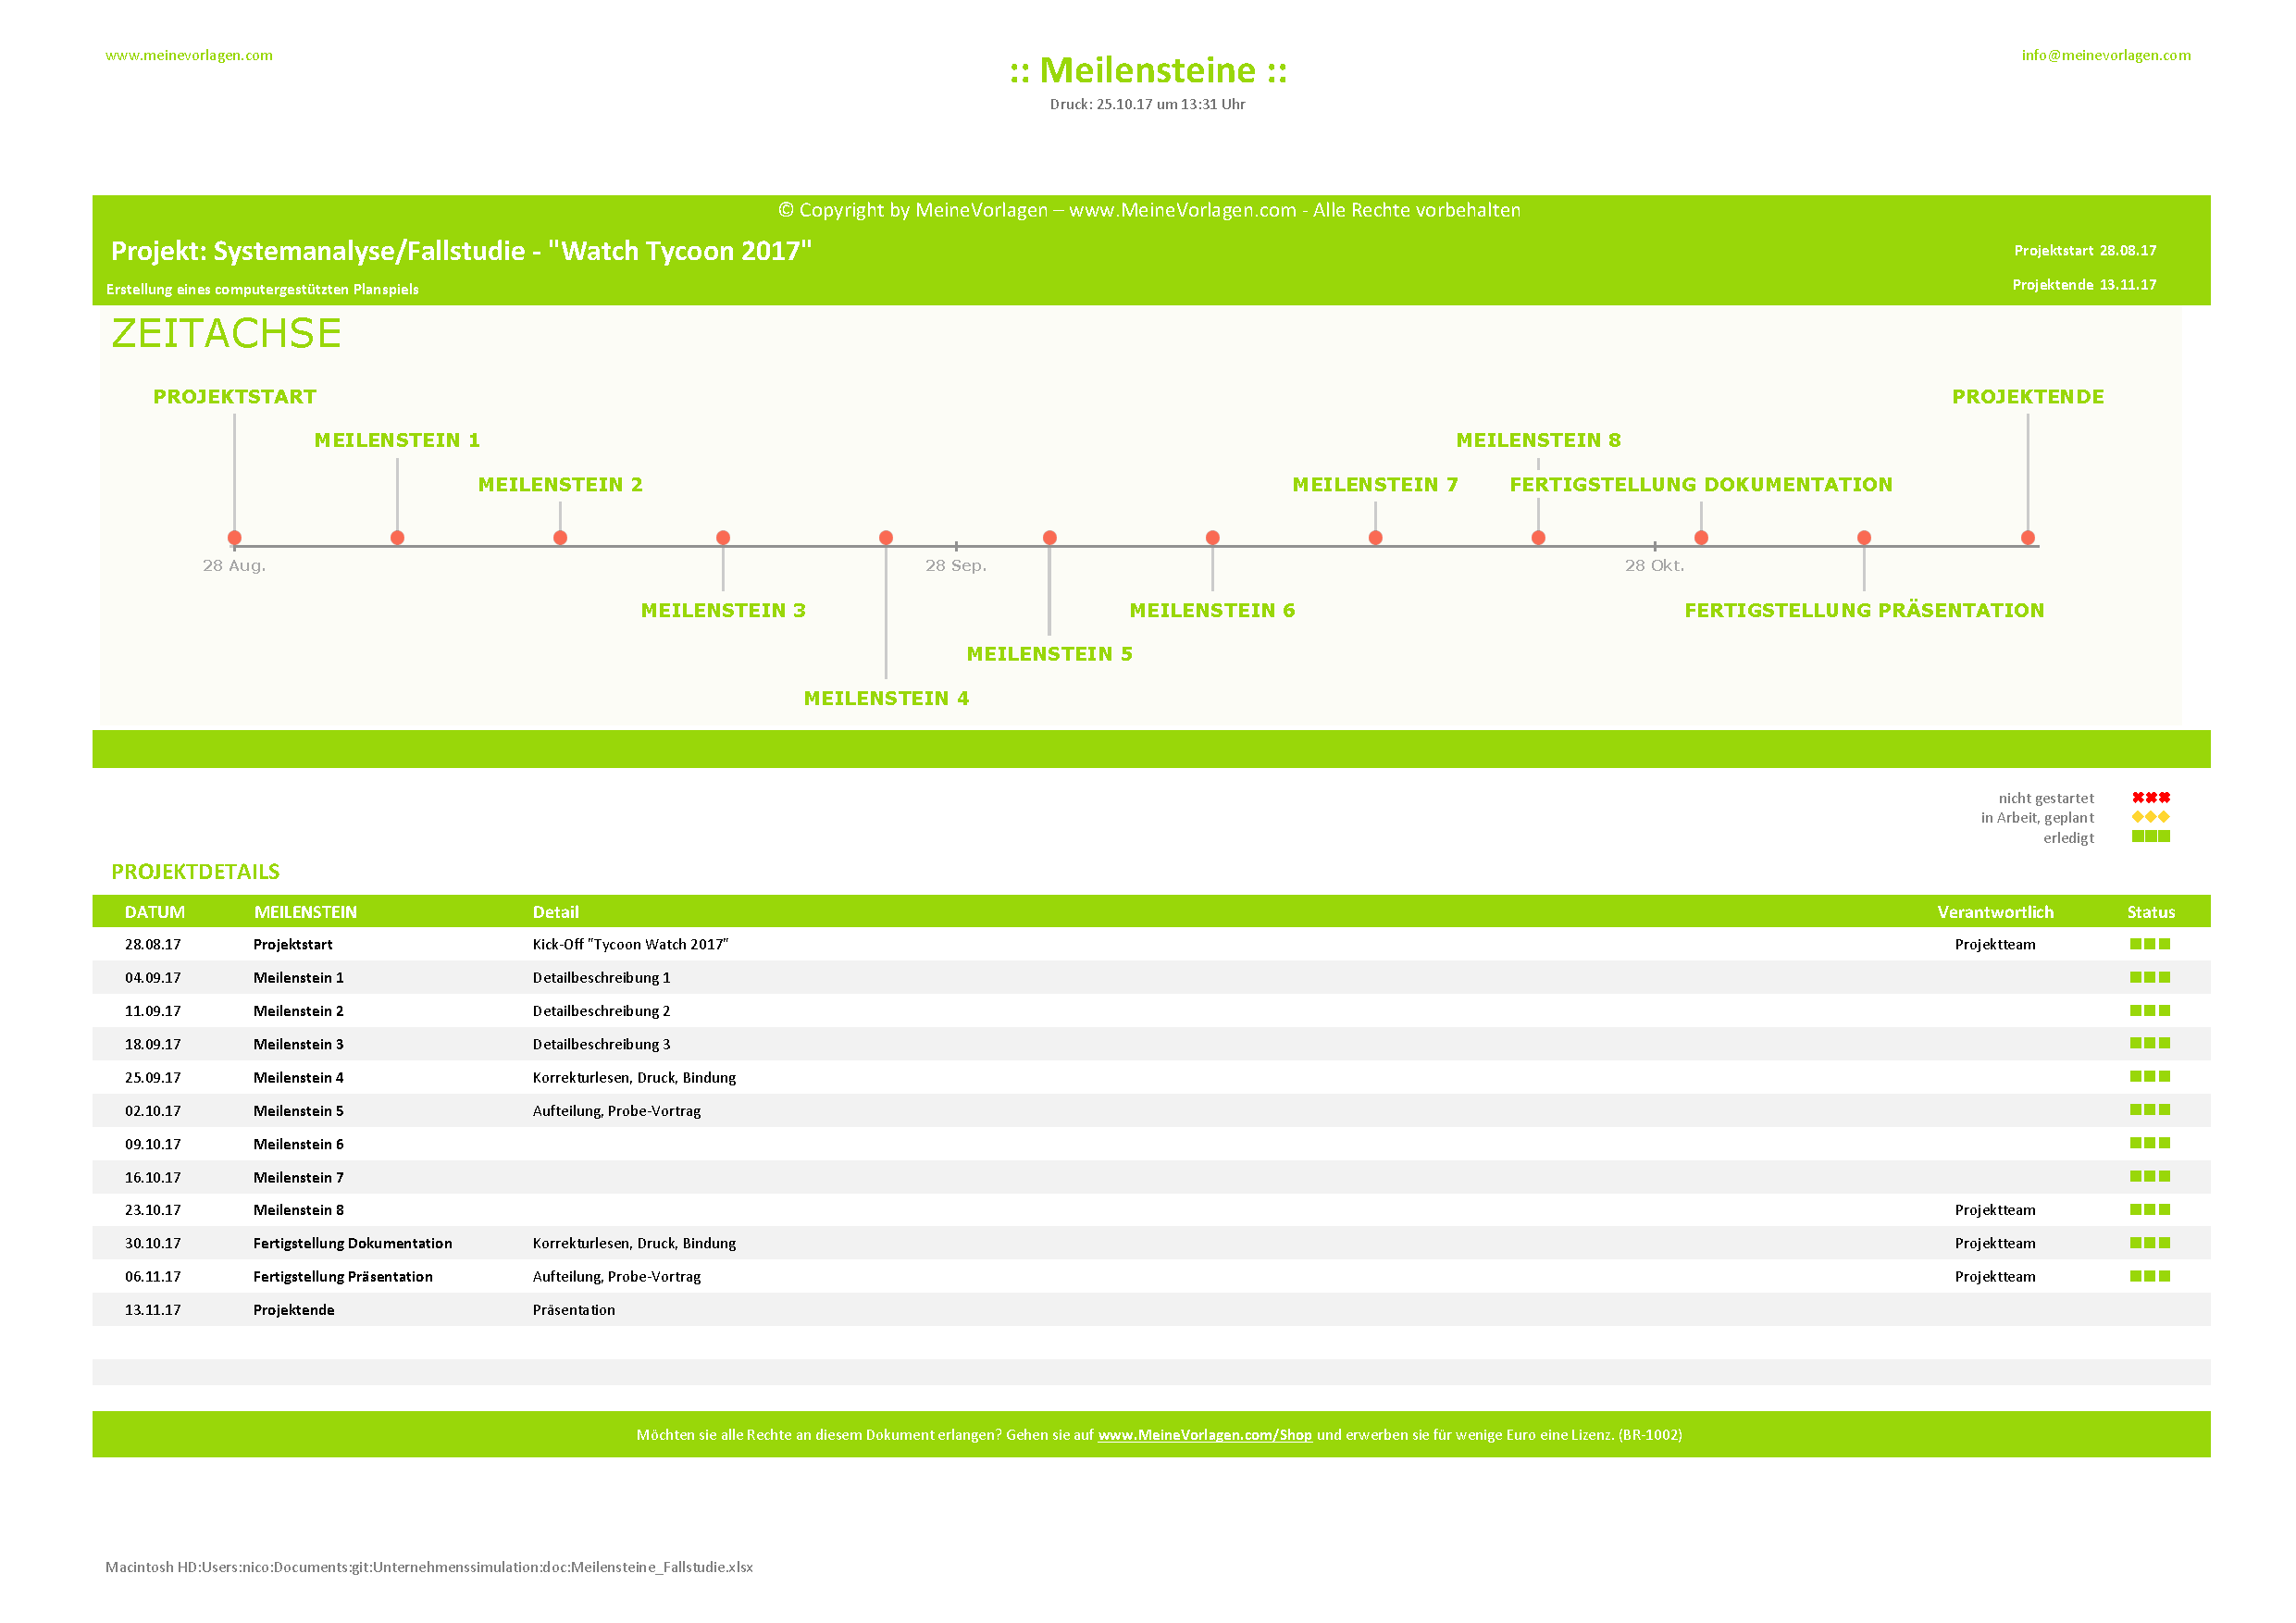
\includegraphics[angle=90, scale=0.45]{img/Meilensteine_Fallstudie.pdf}
	\caption{Meilenstein-Diagramm} \label{fig:abb}
\end{figure}


% 	Ausbaumöglichkeiten
\clearpage
\chapter{Verbesserungs-/Erweiterungsmöglichkeiten}
Während der Durchführungsphase zu diesem Projekt sind einige Verbesserungsmöglichkeiten entstanden, welche aufgrund der Zeit aber nicht mehr realisiert werden konnten. Nachfolgenden finden Sie alle Verbesserungsmöglichkeiten und eine kurze Begründung.
\begin{enumerate}
	\item Erweiterung des Unternehmens um einen HR-Bereich
\begin{itemize}
	\item Wir haben uns schon recht früh gegen einen HR-Bereich entschieden. Gründe hierfür sind zum einen der geringe Bezug zu unserer eigentlichen Aufgabe und zum anderen die mangelnden Funktionen, welche der Bereich für den Spieler mit sich bringen würde. 	
\end{itemize} 
	\item Kreditaufnahme/-tilgung im Einkauf-Bereich
\begin{itemize}
	\item Die Idee war schlichtweg zeitlich nicht mehr möglich.
\end{itemize} 
	\item Speicherung des Spielstands
\begin{itemize}
	\item Da wir uns zu Beginn für ein Hot-Seat Verfahren entschieden haben und das Spiel insgesamt eine kurze Spieldauer hat, sahen wir dies nicht als notwendig an.
\end{itemize} 
	\item Anfälligkeit/Defekte der Produktionsstraßen
\begin{itemize}
	\item Die Idee war schlichtweg zeitlich nicht mehr möglich.
\end{itemize} 
	\item Zufallsereignisse (Krisen, Defekte,...)
\begin{itemize}
	\item Die Idee war schlichtweg zeitlich nicht mehr möglich.
\end{itemize} 
	\item Anzeige der verkauften Uhren (Diagramm) 
\begin{itemize}
	\item Die Idee war schlichtweg zeitlich nicht mehr möglich.
\end{itemize} 	
\end{enumerate}






% 	Fazit/Ausblick
\clearpage
\chapter{Fazit/Ausblick} 

%	Literaturverzeichnis
\ihead{} % Neue Header-Definition
\printbibliography[title=Literaturverzeichnis]
\cleardoublepage

% Der Anhang beginnt hier - jedes Kapitel wird alphabetisch aufgezählt. (Anhang A, B usw.)
\appendix
\ihead{\appendixname~\thechapter} % Neue Header-Definition

% appendix.tex einziehen
\chapter{Testanhang}
\lipsum



\section{Subtestanhang}

\chapter{Noch ein Testanhang}



% Ehrenwörtliche Erklärung ewerkl.tex einziehen
\clearpage
\chapter*{Ehrenwörtliche Erklärung}	

% Wird die folgende Zeile auskommentiert, erscheint die ehrenwörtliche 
% Erklärung im Inhaltsverzeichnis. 

% \addcontentsline{toc}{chapter}{Ehrenwörtliche Erklärung}  

Ich erkläre hiermit ehrenwörtlich: 

\begin{itemize}
	\item dass ich die vorliegende Arbeit mit dem Titel \textit{\DerTitelDerArbeit} selbständig verfasst und
	\item keine anderen als die angegebenen Quellen und Hilfsmittel benutzt habe. 
	\item Ich versichere zudem, dass die eingereichte elektronische Fassung mit der gedruckten Fassung übereinstimmt.
\end{itemize}
Ich bin mir bewusst, dass eine falsche Erklärung rechtliche Folgen haben wird.
\vspace{1cm}
\\
Ort, Datum \hfill Luisa Karl
\\
\\
\\
Ort, Datum \hfill Rebekka Henn
\\
\\
\\
Ort, Datum \hfill Miriam Wolf
\\
\\
\\
Ort, Datum \hfill Erik Schmitt
\\
\\
\\
Ort, Datum \hfill Tillmann Heß
\\
\\
\\
Ort, Datum \hfill Ewald Anselm
\\
\\
\\
Ort, Datum \hfill Nico Feil
 


\end{document}
